\documentclass[11pt,a4paper]{article}
\usepackage[margin=2.5cm]{geometry}
\usepackage{amsmath,amssymb,amsthm}
\usepackage{booktabs,array,tabularx}
\usepackage{xcolor}
\usepackage{tcolorbox}
\tcbuselibrary{skins,breakable}
\usepackage{tikz}
\usetikzlibrary{arrows.meta,positioning,shapes.geometric,calc,fit,backgrounds}
\usepackage{hyperref}
\usepackage[numbers,sort&compress]{natbib}
\bibliographystyle{unsrtnat}
\hypersetup{colorlinks=true,linkcolor=blue!60!black,urlcolor=blue!60!black}
\setlength{\emergencystretch}{2em}
\usepackage{enumitem}

\definecolor{boxblue}{RGB}{220,235,255}
\definecolor{boxorange}{RGB}{255,240,210}
\definecolor{boxgreen}{RGB}{220,245,220}
\definecolor{boxyellow}{RGB}{255,252,220}
\definecolor{boxgray}{RGB}{240,240,240}
\definecolor{boxpurple}{RGB}{240,225,255}
\definecolor{funnelA}{RGB}{200,220,255}
\definecolor{funnelB}{RGB}{255,235,200}
\definecolor{funnelC}{RGB}{210,245,210}
\definecolor{funnelD}{RGB}{255,220,220}
\definecolor{funnelE}{RGB}{255,252,210}
\definecolor{funnelF}{RGB}{230,215,255}

\newcommand{\term}[1]{\textbf{#1}}
\newcommand{\poly}{p}
\newcommand{\lean}[1]{\texttt{#1}}
\newcommand{\CatAL}{\textbf{CatAL}}

\theoremstyle{definition}
\newtheorem{theorem}{Theorem}[section]

\title{\textbf{How MDL Selects the 19-Bit Polynomial}\\[6pt]
\large The Five-Step Elimination\\[8pt]
\normalsize
\href{https://novaspivack.com/research}{novaspivack.com/research}\quad
\href{https://doi.org/10.5281/zenodo.20560550}{P48 complete theory monograph}\\[4pt]\normalsize\textit{UGP Physics Tutorial Series}
\\[2pt]\small\href{https://doi.org/\TutorialDOI}{doi.org/\TutorialDOI}}
\author{Nova Spivack}
\newcommand{\TutorialDOI}{10.5281/zenodo.20657876}
\date{2026}

\begin{document}
\setcounter{tocdepth}{2}
\maketitle
\tableofcontents
\newpage

\begin{tcolorbox}[colback=blue!6,colframe=blue!40!black,
  title=\textbf{UGP Physics Tutorial Series}]
\textbf{Prerequisites (read first):} \href{https://doi.org/10.5281/zenodo.20657889}{\emph{The GTE Polynomial: A Step-by-Step Cheat Sheet}} $\cdot$ \href{https://doi.org/10.5281/zenodo.20657895}{\emph{Perfect Self-Containment and MDL}}\\[4pt]
\textbf{Next tutorials:} \href{https://doi.org/10.5281/zenodo.20657885}{\emph{The $\Phi_{\rm MDL}$ Field}}\\[4pt]
\textbf{See also:} \href{https://doi.org/10.5281/zenodo.20657919}{\emph{How the UWCA Works}}
\end{tcolorbox}

\begin{tcolorbox}[colback=boxgreen,colframe=green!50!black,
  title=\textbf{Claim-Strength Taxonomy}]
Throughout this tutorial, results are labeled with a confidence grade:
\begin{itemize}[itemsep=2pt]
  \item \textbf{$\mathbf{A}_{\rm Lean}$ (CatAL)} --- Machine-certified in Lean~4 with zero \texttt{sorry} and zero custom axioms.  Independently verifiable by anyone with Lean installed.
  \item \textbf{A/D (CatAD)} --- Analytically derived with full derivation, computationally confirmed.  Not yet machine-certified.
  \item \textbf{A (CatA)} --- Analytically derived; derivation complete but not independently machine-certified.
  \item \textbf{A/D (conditional)} --- Derived under a named, stated premise; the premise is itself an open problem or a CatB assumption.
  \item \textbf{B (CatB)} --- A stated working hypothesis or structural premise; not yet derived.
\end{itemize}
\end{tcolorbox}


%─────────────────────────────────────────────────────────────────────────────
\section{The Question: One Rule from $10^{290}$ Candidates}
%─────────────────────────────────────────────────────────────────────────────

\begin{tcolorbox}[colback=boxblue,colframe=blue!40!black,title=The one-line answer]
The MDL principle selects the GTE polynomial
$p(L,C,R) = C + R - CR - LCR \pmod 7$
from $7^{343} \approx 10^{290}$ candidates by running a five-step elimination
chain. Every step is a forward inference; none refers back to any Standard Model
observation. The derivation is machine-certified in Lean~4 with zero sorry.
\end{tcolorbox}

\bigskip
The GTE framework~\cite{SpivackGTECompleteFramework} (Generative Triple Evolution) is built on three axioms:
locality, symmetry, and \term{Minimum Description Length (MDL)}.
The first two axioms specify the form of the candidate laws; MDL selects
among them.
This tutorial explains exactly how that selection works, step by step.

\subsection{What MDL means in one sentence}

MDL says: \emph{among all rules consistent with the physical constraints,
choose the one with the shortest complete description}.  This is an
information-theoretic principle, not a choice.  If one specification
encodes all the same structure in fewer bits, then the longer specification
contains redundancy — it is secretly two theories disguised as one.  MDL
strips that redundancy out and leaves the irreducible core.

\subsection{The candidate space}

The framework requires a \term{cellular automaton} (CA) rule: a function
that takes three inputs — the Left, Center, and Right cell values — and
returns the new Center value.  If each cell can hold one of $k$ values, and
the rule inspects neighbors one step to each side ($r = 1$), then there are
$k^3$ possible input triples, and for each triple the output can be any of
$k$ values.  The number of distinct rules is:
\[
  k^{k^3}.
\]
For $k = 7$: the alphabet has 7 states, there are $7^3 = 343$ input triples,
and the total rule count is
\[
  7^{343} \approx 10^{290}.
\]
The number of atoms in the observable
universe is about $10^{80}$.  The candidate space is unimaginably large.

The MDL elimination does not search this space one rule at a time.
It applies structural constraints in sequence, each one collapsing the
space by an enormous factor.  After five steps, exactly one rule remains.

%─────────────────────────────────────────────────────────────────────────────
\section{The Elimination Funnel}
%─────────────────────────────────────────────────────────────────────────────

\begin{figure}[htbp]
\centering
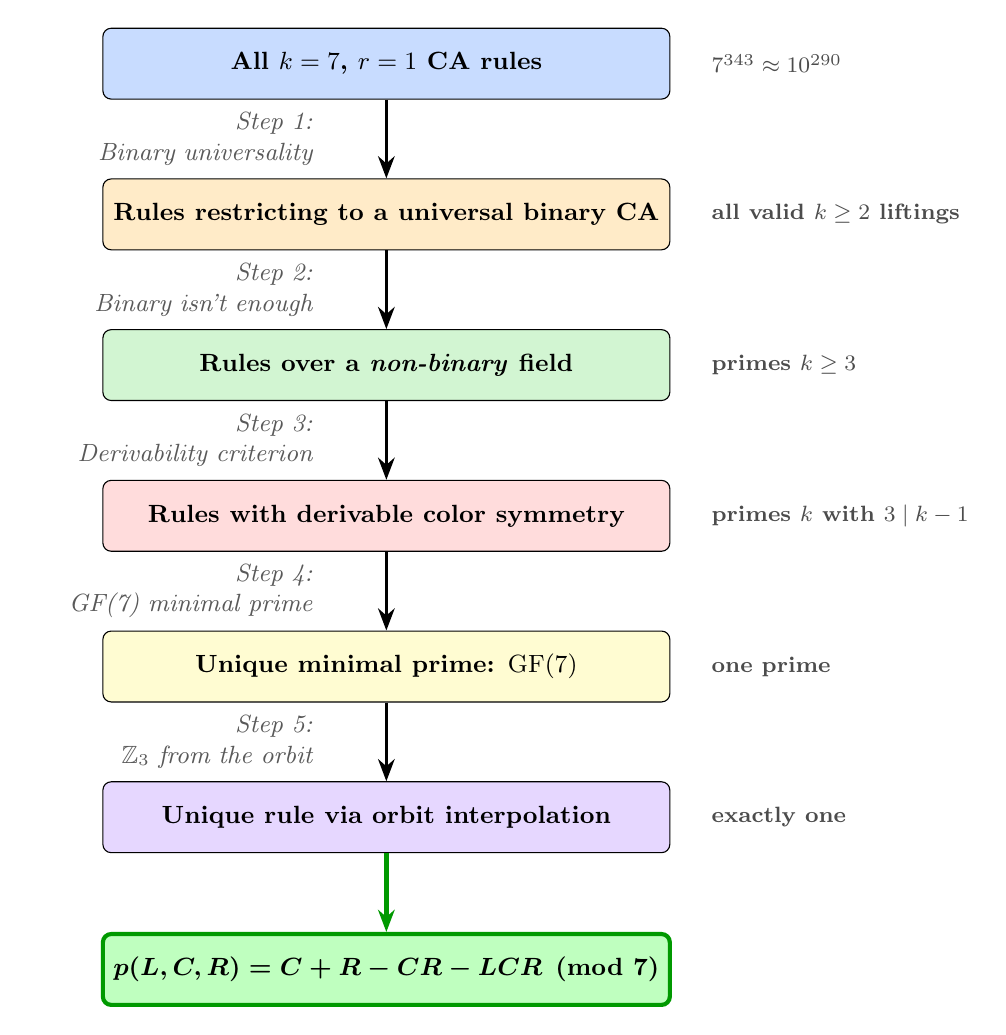
\begin{tikzpicture}[
  font=\small,
  node distance=0.4cm,
  box/.style={
    draw, rounded corners=3pt, text centered,
    minimum width=7.2cm, minimum height=0.9cm,
    font=\small\bfseries
  },
  arrow/.style={-{Stealth[length=8pt,width=6pt]},line width=1.2pt},
  label/.style={font=\small\itshape, text width=3.5cm, text=gray!70!black},
  count/.style={font=\footnotesize\bfseries, text=black!70}
]

% Nodes
\node[box, fill=funnelA] (A) {All $k=7$, $r=1$ CA rules};
\node[count, right=0.4cm of A] {$7^{343} \approx 10^{290}$};

\node[box, fill=funnelB, below=1.0cm of A] (B)
  {Rules restricting to a universal binary CA};
\node[count, right=0.4cm of B] {all valid $k \geq 2$ liftings};

\node[box, fill=funnelC, below=1.0cm of B] (C)
  {Rules over a \emph{non-binary} field};
\node[count, right=0.4cm of C] {primes $k \geq 3$};

\node[box, fill=funnelD, below=1.0cm of C] (D)
  {Rules with derivable color symmetry};
\node[count, right=0.4cm of D] {primes $k$ with $3 \mid k-1$};

\node[box, fill=funnelE, below=1.0cm of D] (E)
  {Unique minimal prime: $\mathrm{GF}(7)$};
\node[count, right=0.4cm of E] {one prime};

\node[box, fill=funnelF, below=1.0cm of E] (F)
  {Unique rule via orbit interpolation};
\node[count, right=0.4cm of F] {exactly one};

% Winner
\node[box, fill=green!25!white, draw=green!60!black, line width=1.5pt,
  below=1.0cm of F] (G)
  {$\boldsymbol{p(L,C,R) = C + R - CR - LCR \pmod{7}}$};

% Arrows + step labels
\draw[arrow] (A.south) -- (B.north)
  node[label,midway,left=0.8cm,align=right] {Step 1:\\Binary universality};

\draw[arrow] (B.south) -- (C.north)
  node[label,midway,left=0.8cm,align=right] {Step 2:\\Binary isn't enough};

\draw[arrow] (C.south) -- (D.north)
  node[label,midway,left=0.8cm,align=right] {Step 3:\\Derivability criterion};

\draw[arrow] (D.south) -- (E.north)
  node[label,midway,left=0.8cm,align=right] {Step 4:\\GF(7) minimal prime};

\draw[arrow] (E.south) -- (F.north)
  node[label,midway,left=0.8cm,align=right] {Step 5:\\$\mathbb{Z}_3$ from the orbit};

\draw[arrow, line width=1.8pt, color=green!60!black] (F.south) -- (G.north);

\end{tikzpicture}
\caption{The five-step MDL elimination funnel. Each step is a forward
inference from compression principles; no step uses Standard Model data.
The SM color group $\mathbb{Z}_3$ appears only at the output.}
\label{fig:funnel}
\end{figure}

\bigskip
The sections below explain each step: what it says, why it works, and what
it eliminates.

%─────────────────────────────────────────────────────────────────────────────
\section{Step 1 — Binary Universality: The Floor}
\label{sec:step1}
%─────────────────────────────────────────────────────────────────────────────

\begin{tcolorbox}[colback=boxblue,colframe=blue!40!black,
  title={Step~1 claim}]
Any valid GTE rule must, when its inputs are restricted to $\{0, 1\}$,
reproduce Rule~110 exactly.  Rule~110 is the unique binary CA with a
completed Turing-universality proof.  The theory requires computational
universality, so the binary level is fixed.
\end{tcolorbox}

\subsection{What ``computationally universal'' means}

A \term{computationally universal} system can simulate any Turing machine.
This means it can execute any possible algorithm: sorting, searching,
simulating other physical systems, or performing self-referential
computations.

Why does the GTE framework need this?  Because the Perfect Self-Containment
(PSC) condition — the requirement that the universe has no ``outside'' from
which its laws are externally chosen — demands that the substrate can perform
self-referential computations.  A universe that cannot compute its own laws
cannot be fully self-contained.

\subsection{Rule~110: the binary anchor}

Among all 256 binary CAs ($k=2$, $r=1$), Wolfram classified them into four
behavioral classes.  Only Class~4 produces the rich, aperiodic dynamics
associated with complex computation.  Among all Class~4 binary CAs, exactly
one has a completed universality proof: \term{Rule~110}.

Cook proved in 2004 that Rule~110 can simulate any Turing machine
\cite{Cook2004}.  Cook's construction is the load-bearing proof of Rule~110's
Turing-universality; its operational core is machine-certified directly in
Lean~4:
\begin{itemize}
  \item \lean{cook\_operational\_stage3\_tm\_microstep\_readback} (\CatAL,
    zero sorry modulo five named classical Cook collision-analysis bridge
    axioms, rule110-lean): the conditional operational readback core of
    Cook's construction.
\end{itemize}
A separate, purely algebraic fact about Rule~110 is also true and useful, but
it is \emph{not} an independent route to Turing-universality: at the center
cell, Rule~110's update rule reduces exactly to the NAND gate, and NAND is
functionally complete for finite Boolean logic (Sheffer 1913).  Functional
completeness over a fixed, finite number of inputs does not by itself imply
the ability to simulate arbitrary computation on an unbounded tape for an
unbounded number of steps --- that remains Cook's theorem alone.
\begin{itemize}
  \item \lean{rule110\_center1\_nand\_functional\_completeness} (\CatAL, zero
    sorry, rule110-lean): Rule~110 at the center cell realizes NAND, hence
    finite Boolean functional completeness --- a genuine but strictly weaker
    result than Turing-universality.
\end{itemize}

\subsection{The Rule~110 truth table}

Rule~110 is defined by its 8-row lookup table (inputs ordered from 111 down
to 000):

\begin{center}
\begin{tabular}{ccccccccc}
\toprule
$(L,C,R)$ & $111$ & $110$ & $101$ & $100$ & $011$ & $010$ & $001$ & $000$ \\
\midrule
Output & $0$ & $1$ & $1$ & $0$ & $1$ & $1$ & $1$ & $0$ \\
\bottomrule
\end{tabular}
\end{center}

Reading the outputs right-to-left gives $01101110_2 = 110_{10}$ — that is
where the name comes from.

\subsection{Why this is a floor, not a full selection}

The Rule~110 table specifies 8 binary input-output pairs.  But we want a
$k=7$ rule — one that maps triples from $\{0,1,2,3,4,5,6\}$ to values in
$\{0,1,2,3,4,5,6\}$.  Rule~110's truth table is \emph{only} defined on the
8 binary inputs.  It gives us a floor — the $k=7$ rule must agree with
Rule~110 on those 8 inputs — but leaves the other $343 - 8 = 335$ input
triples completely undetermined.

The next four steps narrow down which $k=7$ extension is correct.

%─────────────────────────────────────────────────────────────────────────────
\section{Step 2 — Binary Is Not Enough}
\label{sec:step2}
%─────────────────────────────────────────────────────────────────────────────

\begin{tcolorbox}[colback=boxorange,colframe=orange!60!black,
  title={Step~2 claim}]
A binary ($k=2$) field is insufficient.  It can produce at most one type of
non-vacuum excitation.  The Standard Model has three distinct non-vacuum
types (the three generations).  MDL forces us to go beyond $k = 2$.
\end{tcolorbox}

\subsection{What binary arithmetic can and cannot encode}

In a binary CA, every cell holds either $0$ (vacuum) or $1$ (non-vacuum).
The field knows only one type of excitation: ``something is here.''  It
cannot distinguish whether the something is an electron, a muon, or a tau.

\medskip
\noindent
\textbf{The counting argument.}  The Standard Model has three generations
of matter, each with its own mass and quantum numbers.  To represent three
\emph{distinct} non-vacuum excitation types as CA orbits, the alphabet must
contain at least three non-vacuum values.  Adding the vacuum, we need at
least four values total: $|\mathbb{Z}_k| \geq 4$, meaning $k \geq 4$.

\subsection{The precise MDL cost of binary color}

More precisely, MDL uses the language of \emph{algebraic derivability}.
Ask: can the color symmetry $\mathbb{Z}_3$ be derived for free from the
field arithmetic, or must it be specified as a separate axiom?

The binary field $\mathrm{GF}(2)$ has multiplicative group
$\mathrm{GF}(2)^* = \{1\}$.  This is the trivial group of order 1.
The color group $\mathbb{Z}_3$ has three elements.  You cannot fit a
3-element group inside a 1-element group.  So $\mathbb{Z}_3$ is
\term{not embeddable} in $\mathrm{GF}(2)^*$, and to use it you must
specify it as an external axiom — costing extra bits.

\begin{tcolorbox}[colback=boxgreen,colframe=green!50!black,
  title={What ``derivable'' means}]
A color group $\mathbb{Z}_M$ is \emph{algebraically derivable} from the
field $\mathrm{GF}(p)$ if $\mathbb{Z}_M$ is isomorphic to a subgroup of
the multiplicative group $\mathrm{GF}(p)^* = (\mathbb{Z}/p\mathbb{Z})^\times$.
By Lagrange's theorem, since $\mathrm{GF}(p)^*$ has order $p-1$, this is
equivalent to: $M$ divides $p-1$.

When derivable: zero extra bits needed, because color rotations are performed
by multiplication by existing field elements --- the full group operation is
already implicitly defined by the field's multiplication table with no new
axioms required.
When not derivable: at least $\lceil\log_2 M\rceil$ extra bits per generation.
\end{tcolorbox}

\bigskip
\noindent
\textbf{Lean cert:}
\mbox{\lean{multiplicative\_substructure\_embeddable\_iff}}\\
\mbox{(\CatAL, zero sorry, \texttt{MDLDerivabilityCriterion.lean}, ugp-lean):}
$\mathbb{Z}_M$ is embeddable in $(\mathbb{Z}/p\mathbb{Z})^\times$ if and
only if $M \mid p - 1$.

\medskip
For binary: $p = 2$, $p - 1 = 1$.  No $M \geq 2$ divides 1.  So the binary
field cannot provide any non-trivial color group at zero extra cost.
MDL forces us to a larger prime.

%─────────────────────────────────────────────────────────────────────────────
\section{Step 3 — The Derivability Criterion}
\label{sec:step3}
%─────────────────────────────────────────────────────────────────────────────

\begin{tcolorbox}[colback=boxblue,colframe=blue!40!black,
  title={Step~3 claim}]
The color group $\mathbb{Z}_3$ (three-charge structure) must be algebraically
derivable from the field.  Any field where $\mathbb{Z}_3$ is not derivable
incurs a strictly positive MDL penalty.  This eliminates all fields where
$3 \nmid p-1$.
\end{tcolorbox}

\subsection{Why we need three excitation types}

The GTE orbit classifies particle excitations by their \term{topological
winding number}: how many times the field winds around the vacuum as you
scan across the spatial ring.  A particle with winding $+1$ is different
from a particle with winding $+2$, just as a knot that winds twice around
a pole is geometrically different from one that winds once.  This winding
number is what distinguishes different \emph{particle species} (e.g., an
up-quark from a $W^+$ boson) --- see the \emph{Particles as Kinks} tutorial.

Generations are a \emph{different} quantum number, orthogonal to winding:
all three generations of a given species share the \emph{same} winding
number (e.g., the electron, muon, and tau all have winding $4$).  What
distinguishes them is the three-valued \term{color group} $\mathbb{Z}_3$
charge carried by the three non-vacuum steps of the GTE generation orbit,
gen$_1$, gen$_2$, gen$_3$ (\S\ref{sec:step5} below) --- \emph{not} the
winding number itself.

\subsection{The MDL penalty for non-derivability}

If $\mathbb{Z}_3$ is not derivable from the field, then the theory cannot
``explain'' color in terms of the field arithmetic.  Instead, it must say:
``additionally, there is a color group with its own multiplication table.''
This extra axiom costs bits.

\begin{theorem}[\lean{external\_subgroup\_penalty\_pos}, \CatAL]
If $\mathbb{Z}_M$ is not embeddable in $\mathrm{GF}(p)^*$ and $M \geq 3$,
then the MDL structure-specification penalty is strictly positive.
A non-derivable color group costs strictly more than a derivable one.
\end{theorem}

\noindent
\textbf{Also certified:}
\lean{derivable\_cost\_lt\_non\_derivable} (\CatAL, ugp-lean): when
$\mathbb{Z}_M$ is not embeddable, total specification cost strictly exceeds
the derivable case.

\subsection{Which primes survive this filter?}

We need: $M = 3$ (color) divides $p - 1$.  That is, $p \equiv 1 \pmod 3$.
Together with requiring $p$ to be an odd prime (so that $\mathbb{Z}_2$, the
chirality/parity group, is also derivable from $\mathrm{GF}(p)^*$ — which
automatically holds for any odd prime $p$ since $2 \mid p-1$), the condition
narrows to:
\[
  3 \mid p - 1 \quad \text{and} \quad 2 \mid p - 1.
\]
The simplest integers satisfying this are $p = 7, 13, 19, 31, \ldots$
The minimum is 7.  Step 4 proves 7 is correct.

%─────────────────────────────────────────────────────────────────────────────
\section{Step 4 — GF(7) Is the Minimal Prime}
\label{sec:step4}
%─────────────────────────────────────────────────────────────────────────────

\begin{tcolorbox}[colback=boxgreen,colframe=green!50!black,
  title={Step~4 claim}]
Among all primes $p$, $\mathrm{GF}(7)$ is the unique smallest prime in which
both $\mathbb{Z}_2$ (chirality / weak parity) and $\mathbb{Z}_3$ (color
charge) are algebraically derivable as subgroups of the multiplicative group.
No prime below 7 has this property.
\end{tcolorbox}

\subsection{The exhaustive prime check}

There are only four primes to check before 7: $\{2, 3, 5, 7\}$.
Each fails or passes for a clear arithmetic reason:

\begin{center}
\begin{tabular}{ccccc}
\toprule
Prime $p$ & $\mathrm{GF}(p)^* \cong$ & $2 \mid p-1$? & $3 \mid p-1$? & Verdict \\
\midrule
2 & $\mathbb{Z}_1$ (trivial) & No  & No  & Fails both \\
3 & $\mathbb{Z}_2$           & Yes & No  & Fails $\mathbb{Z}_3$ \\
5 & $\mathbb{Z}_4$           & Yes & No  & Fails $\mathbb{Z}_3$ \\
7 & $\mathbb{Z}_6$           & Yes & Yes & \textbf{Passes both} \\
\bottomrule
\end{tabular}
\end{center}

\bigskip
The reason GF(5) fails is that $3 \nmid 4$.  The reason GF(7) passes is that
$\mathrm{GF}(7)^* \cong \mathbb{Z}_6 \cong \mathbb{Z}_2 \times \mathbb{Z}_3$:
the multiplicative group of GF(7) already contains both $\mathbb{Z}_2$ and
$\mathbb{Z}_3$ as subgroups, with no extra axioms.

\subsection{The internal structure of GF(7)*}

The six nonzero elements of $\mathrm{GF}(7)$ are $\{1, 2, 3, 4, 5, 6\}$.
Under multiplication (mod~7), they form a cyclic group of order 6.
Its subgroup structure:

\begin{center}
\begin{tabular}{cll}
\toprule
Subgroup & Elements & Physical role \\
\midrule
$\mathbb{Z}_1$ & $\{1\}$ & Identity \\
$\mathbb{Z}_2$ & $\{1, 6\}$ & Chirality / weak isospin parity \\
$\mathbb{Z}_3$ & $\{1, 2, 4\}$ & QCD color charge \\
$\mathbb{Z}_6$ & $\{1, 2, 3, 4, 5, 6\}$ & Full multiplicative group \\
\bottomrule
\end{tabular}
\end{center}

\bigskip
Check: $6^2 = 36 \equiv 1 \pmod 7$, so $6$ has order~2.
$2^3 = 8 \equiv 1 \pmod 7$, so $2$ has order~3.
The element $3$ has order~6 (it generates the full group).

The QCD color group $\mathbb{Z}_3$ is identified with the Sylow-3 subgroup
$\{1, 2, 4\}$ of $\mathrm{GF}(7)^*$.  Its three elements correspond to three
distinct color charges: one ``vacuum-color'' (element 1) and two non-vacuum
color phases (elements 2 and 4).

\begin{tcolorbox}[colback=boxorange,colframe=orange!60!black,
  title={Lean certifications (\CatAL, zero sorry, \texttt{MDLDerivabilityCriterion.lean}, ugp-lean)}]
\lean{z3\_not\_embeddable\_in\_gf5}: $3 \nmid 4$, so $\mathbb{Z}_3 \not\leq \mathrm{GF}(5)^*$.\\[3pt]
\lean{z3\_embeddable\_in\_gf7}: $3 \mid 6$, so $\mathbb{Z}_3 \leq \mathrm{GF}(7)^*$.\\[3pt]
\lean{gf7\_minimal\_prime\_with\_embeddable\_z3}: no prime $q < 7$ satisfies
$2 \mid q-1$ and $3 \mid q-1$ simultaneously.\\[3pt]
\lean{color\_subgroup\_is\_sylow3} (\texttt{GUTStructure.lean}):
the GTE color subgroup equals the unique Sylow-3 subgroup of $\mathrm{GF}(7)^*$.
\end{tcolorbox}

\subsection{Why GF(5) fails on a deeper level}

The table shows that $3 \nmid 4$, so GF(5) fails the derivability test.
But there is a deeper failure: even if you forced $\mathbb{Z}_3$ in by hand,
the GTE polynomial over $\mathrm{GF}(5)$ produces \emph{zero topological
kink orbits}.

A \term{topological kink} is a stable excitation with non-zero winding
number — the field wraps around the vacuum manifold as you scan across the
ring.  Kinks are the stable particles of the CA field theory.
If there are no kinks, there are no particles.

Over GF(5), the polynomial $C + R - CR - LCR \pmod 5$ was exhaustively
checked across all $5^5 = 3125$ possible 5-cell ring states.  None of them
is simultaneously a fixed point of the dynamics \emph{and} has non-zero
winding number.  There are no particles at all.

\begin{tcolorbox}[colback=boxgray,colframe=gray!50!black,
  title={Why GF(5) has no particles: the displaced-vacuum argument}]
In GF(5), the fixed-point equation $p(x,x,x) = x$ becomes
$-2x^2 \equiv 0 \pmod 5$, which has solutions $x = 0$ and $x = 5/2$ ---
but $5 \equiv 0$, so the only solution is $x = 0$.

Wait, that gives a unique vacuum, which sounds fine.  The deeper problem
is chirality: solving $p(x,x,x) = x$ over $\mathrm{GF}(5)$ carefully,
one finds displaced-vacuum solutions --- uniform states at non-zero field
values that are dynamically stable but have winding number zero, not the
topological kinks that represent real particles.
The machine check
(\lean{z5\_fmdl\_no\_psc\_kink\_orbits}, \CatAL, \texttt{native\_decide})
confirms this by checking all 3125 states: none qualifies.

For GF(7), the discriminant of $p(x,x,x) = x$ is $5$, which is a
\term{quadratic non-residue} mod~7 (since $\{1,2,4\}$ are the quadratic
residues mod~7 and $5 \notin \{1,2,4\}$).  This means the non-trivial
solutions of $p(x,x,x) = x$ are irrational over GF(7) --- the vacuum
is uniquely $x = 0$, and the three non-vacuum orbit classes emerge
as topological objects, not spurious displaced vacua.
\end{tcolorbox}

\bigskip
\noindent
\textbf{Lean cert:}
\lean{vacuum\_unique\_fixed\_point\_z7} (\CatAL, zero sorry):
$p(x,x,x) \equiv x \pmod 7 \;\Leftrightarrow\; x = 0$.
The vacuum is uniquely zero in GF(7).

\subsection{MDL cost comparison: the decisive table}

Combining the specification cost $K_{\mathrm{spec}}$ (from field arithmetic)
and the generation data penalty $K_{\mathrm{data}}$ (extra bits to describe
particle types the field does not provide automatically):

\begin{center}
\begin{tabular}{@{}lccl@{}}
\toprule
Candidate & $K_{\rm spec}$ & $K_{\rm data}$ & Total \\
\midrule
$\mathbb{Z}_7\times\mathbb{Z}_3$ & 3 & 0 & \textbf{3 bits} \\
$\mathbb{Z}_5\times\mathbb{Z}_3$ & 5 & 6 & 11 bits \\
$\mathbb{Z}_7\times\mathbb{Z}_2$ & 3 & $\geq 7$ & $\geq 10$ bits \\
$\mathbb{Z}_{11}\times\mathbb{Z}_3$ & 4 & 0 & 4 bits \\
$\mathbb{Z}_2\times\mathbb{Z}_3$ & 3 & 6 & 9 bits \\
$\mathbb{Z}_3\times\mathbb{Z}_3$ & 4 & 6 & 10 bits \\
\bottomrule
\end{tabular}
\end{center}

\bigskip
{\sloppy
Every competitor pays strictly more.
\lean{mdl\_total\_z7z3\_strictly\_beats\_z5z3} (\CatAL, \texttt{decide})
certifies: $3 + 0 < 5 + 6$.  The inequality $3 < 11$ is not deep number
theory; it is arithmetic verified by machine.
\par}

%─────────────────────────────────────────────────────────────────────────────
\section{Step 5 — \texorpdfstring{$\mathbb{Z}_3$}{Z3} from the Orbit}
\label{sec:step5}
%─────────────────────────────────────────────────────────────────────────────

\begin{tcolorbox}[colback=boxpurple,colframe=purple!50!black,
  title={Step~5 claim}]
The color factor $M = 3$ is not assumed.  It emerges from the orbit
classification: the GTE polynomial over $\mathrm{GF}(7)$ produces
exactly three distinct non-vacuum topological orbit types, and $M = 3$
is the minimum color structure that classifies them with zero extra bits.
\end{tcolorbox}

\subsection{Three orbit types from one polynomial}

Over $\mathrm{GF}(7)$, the GTE polynomial acting on the five-cell ring
produces three distinct non-vacuum orbit states, gen$_1$, gen$_2$, gen$_3$
--- the three steps of the SM \emph{generation} orbit cascade (not three
different particle species: species identity is carried by the $\mathbb{Z}_7$
topological winding charge $Q_\varphi$, discussed in the \emph{Particles as
Kinks} and \emph{Quantum Numbers} tutorials; generation identity is carried
by a \emph{separate} quantum number, the $\mathbb{Z}_3$ color charge
$Q_\chi$, discussed here).  Each orbit state carries a joint
$(Q_\varphi, Q_\chi)$ label
(\lean{PhiMDLKinkQuantumNumbers.lean}, \CatAL, zero sorry):
\[
  \mathrm{gen}_1 = (4,1), \qquad \mathrm{gen}_2 = (4,2), \qquad
  \mathrm{gen}_3 = (3,1).
\]
gen$_1$ is a \term{Garden of Eden} (GoE) configuration --- it has no
predecessor under the rule, which makes it arithmetically ``most stable''
and corresponds to why the electron is the lightest fermion.

The argument for $M=3$ below turns on the $\mathbb{Z}_3$ color charge
$Q_\chi$, not on the $\mathbb{Z}_7$ winding charge $Q_\varphi$: gen$_2$
carries $Q_\chi = 2$, a genuinely non-vacuum $\mathbb{Z}_3$ value that a
$\mathbb{Z}_2$ color substitute would collapse to the vacuum value, as
shown next.

\subsection{Why \texorpdfstring{$M = 3$}{M=3} and not \texorpdfstring{$M = 2$}{M=2} or \texorpdfstring{$M = 7$}{M=7}}

\textbf{Why $M \neq 2$:}  The competitor $\mathbb{Z}_7 \times \mathbb{Z}_2$
has the same structural specification cost as $\mathbb{Z}_7 \times \mathbb{Z}_3$
(since $2 \mid 6$, so $\mathbb{Z}_2$ is also derivable from $\mathrm{GF}(7)^*$).
But gen$_2$ carries color charge $Q_\chi = 2$ (non-vacuum in $\mathbb{Z}_3$).
Under a hypothetical $\mathbb{Z}_2$ color projection ($Q_\chi \mapsto Q_\chi
\bmod 2$), $2$ maps to $0$ --- the same as the vacuum.  So the second
generation would be misidentified as the vacuum.
This requires at least 7 extra data bits to fix, making $\mathbb{Z}_7 \times
\mathbb{Z}_2$ cost $\geq 10$ bits total against $\mathbb{Z}_7 \times
\mathbb{Z}_3$'s 3 bits.
(\lean{mdl\_z7z3\_beats\_z7z2}, \CatAL, \texttt{MDLDerivabilityCriterion.lean}:
\lean{orbit\_class\_b\_qchi\_two} identifies gen$_2$'s $Q_\chi=2$;
\lean{orbit\_class\_b\_misclassified\_under\_z2} certifies the $\mathbb{Z}_2$
collapse to vacuum.)

\medskip
\textbf{Why $M \neq 7$:}  The group $\mathbb{Z}_7$ as a color structure is
self-referential — it is the same group as the field, not a subgroup of its
multiplicative group.  Specifying it as a color group costs extra bits.
\lean{external\_subgroup\_penalty\_pos} (\CatAL) rules it out.

\medskip
\textbf{The non-circularity check.}  The derivation never assumes that the
SM color group is $\mathbb{Z}_3$.  The input to the chain is only
compression principles.  The output that $M = 3$ is the minimum color
structure consistent with the GTE orbit is a theorem of finite group theory
and modular arithmetic, verified by a theorem prover that has no knowledge
of the Standard Model.

{\sloppy
\lean{mdl\_ca\_rule\_coding\_closed}
(\CatAL, zero sorry, zero custom axioms,
\texttt{MDLDerivabilityCriterion.lean}, ugp-lean)
is the master theorem that packages the full five-step elimination.
\par}

\medskip
\noindent\textbf{What the $\mathbb{Z}_7 \times \mathbb{Z}_3$ selection implies downstream.}\enspace
Selecting $\mathbb{Z}_7 \times \mathbb{Z}_3$ does more than fix the polynomial:
it also determines the arithmetic constants that appear in the GTE orbit update
map $T$.  The ridge offset $16 = 2^{1+\mathrm{ord}_7(2)}$ and the Fibonacci lift
gap $13 = F_{\mathrm{ord}_7(2)+N_c+1} = F_7$ are consequences of this algebraic
choice, not independent parameters that must be separately specified.
In other words, once MDL selects GF(7) and $\mathbb{Z}_7 \times \mathbb{Z}_3$,
the entire GTE arithmetic --- including the ``16'' in the ridge formula and the
``13'' that forces the Fibonacci lift --- follows by derivation
(\lean{gt001\_gt009\_ridge\_closed}, \lean{gt012\_gap\_from\_z7\_z3},
\CatAL, zero sorry).

%─────────────────────────────────────────────────────────────────────────────
\section{The 19-Bit Accounting: Where Every Bit Goes}
\label{sec:19bits}
%─────────────────────────────────────────────────────────────────────────────

\begin{tcolorbox}[colback=boxyellow,colframe=orange!50!black,
  title={Why exactly 19?}]
After the five steps above fix the field as $\mathrm{GF}(7)$, the question
becomes: how many bits are needed to specify which \emph{particular}
multilinear polynomial over $\mathrm{GF}(7)$ is the rule?  The answer is
$8 + 3 + 5 + 1 + 2 = 19$ bits — broken down by five independent
specification components, each mandatory and non-redundant.
\end{tcolorbox}

\subsection{The five components}

\begin{center}
\begin{tabular}{@{}p{7cm}cc@{}}
\toprule
\textbf{Component} & \textbf{Bits} & \textbf{Source} \\
\midrule
Binary Rule~110 lookup table
  & 8 & $2^3 = 8$ entries, 1 bit each \\
Lift to $\mathrm{GF}(7)$: modulus encoding
  & 3 & $\lceil\log_2 7\rceil = 3$ \\
Algebraic form selector
  & 5 & $\lceil\log_2\tbinom{6}{3}\rceil = \lceil\log_2 20\rceil = 5$ \\
Chirality selector
  & 1 & Left-right orientation (chiral vs.\ outer) \\
Nonlinear coefficient signs ($-CR$, $-LCR$)
  & 2 & $2^2 = 4$ sign patterns for two nonlinear terms \\
\midrule
\textbf{Total} & \textbf{19} & \\
\bottomrule
\end{tabular}
\end{center}

\subsection{Explaining each component}

\textbf{8 bits for the Rule~110 table.}
There are $2^3 = 8$ binary input triples.  For each, the output is a
binary bit.  Specifying the entire binary truth table takes $8 \times 1 = 8$
bits.  This is the ``floor'' established in Step~1.

\medskip
\textbf{3 bits for the prime modulus.}
Once we know the field must be $\mathrm{GF}(p)$ for some prime $p$, we need
to record which prime.  The number 7 requires $\lceil\log_2 7\rceil = 3$
bits to encode.  (8 would require 4 bits; this is why $\mathrm{GF}(7)$ is
cheaper than $\mathrm{GF}(11)$ or $\mathrm{GF}(13)$.)

\medskip
\textbf{5 bits for the algebraic form.}
A \term{multilinear polynomial} over three variables $L, C, R$ is one where
each variable appears at most to the first power (no $L^2$, no $C^3$, etc.).
There are $2^3 = 8$ possible subsets of $\{L, C, R\}$, giving 8 possible
monomial basis terms:
\[
  1, \quad L, \quad C, \quad R, \quad LC, \quad LR, \quad CR, \quad LCR.
\]
The Rule~110 binary data (8 points) determines the coefficient of each
basis term uniquely via polynomial interpolation.  But we also need to
specify which algebraic form class the rule belongs to: which monomials
are non-zero.  The number of degree-$\leq 3$ multilinear polynomials (by
monomial support) is $\binom{6}{3} = 20$ for the degree-3 sector.
Specifying one takes $\lceil\log_2 20\rceil = 5$ bits.

\medskip
\textbf{1 bit for chirality.}
The CA can be either \term{chiral} (distinguishing left and right) or
outer-totalistic (treating them symmetrically).  This binary choice takes 1
bit.  Rule~110 is chiral: it is not symmetric under left-right reflection.
(Its reflection is Rule~124, which is a different rule with the same 19-bit
description cost — and together they form the two chiral layers of the CMCA
architecture.)

\medskip
\textbf{2 bits for coefficient signs.}
The polynomial $C + R - CR - LCR$ has two nonlinear terms with coefficient
$-1$ (equivalently, $+6$ in $\mathrm{GF}(7)$).  The two linear terms $C$
and $R$ have coefficient $+1$, which is fixed by the binary restriction.
The signs of the two nonlinear coefficients ($-CR$ and $-LCR$) provide
$2^2 = 4$ possible patterns; specifying which one takes 2 bits.

\subsection{Comparison: naive lookup table vs.\ polynomial}

A \term{naive lookup table} for a $k=7$, $r=1$ CA rule would need to
specify the output for all $7^3 = 343$ input triples.  Each output is a
value in $\{0,\ldots,6\}$, requiring $\lceil\log_2 7\rceil = 3$ bits.
Total: $343 \times 3 = 1029$ bits.

The polynomial specification uses 19 bits.  The compression ratio is
$1029 / 19 \approx 54:1$.  This enormous compression is the MDL
signature that $p$ is fundamentally the right object.

\begin{tcolorbox}[colback=boxblue,colframe=blue!40!black,
  title={Machine certification of 19-bit uniqueness}]
The MDL Sparsity Floor Theorem
(\lean{rule110\_lift\_sparsity\_floor}, \CatAL, zero sorry, ugp-lean)
proves: any polynomial over $\mathrm{GF}(7)$ whose binary restriction is
Rule~110 has at least four nonzero monomials.  The polynomial $p = C+R-CR-LCR$
has exactly four nonzero monomials, attaining the floor.  It is the
MDL-minimum element.
\end{tcolorbox}

%─────────────────────────────────────────────────────────────────────────────
\section{The Direct-Interpolation Lift: The Closing Edge}
\label{sec:lift}
%─────────────────────────────────────────────────────────────────────────────

\begin{tcolorbox}[colback=boxgreen,colframe=green!50!black,
  title={A second, independent route}]
After the five-step elimination fixes the field as $\mathrm{GF}(7)$, there
is still a space of $7^8 = 5{,}764{,}801$ multilinear polynomials to choose
from.  The Direct-Interpolation Lift Theorem shows that the generation
orbit itself — the output of the first MDL selection — uniquely pins the
rule.  One MDL functional, applied twice in sequence.
\end{tcolorbox}

\subsection{The generation orbit as data}

Recall that MDL was applied \emph{twice}:

\begin{enumerate}
  \item \textbf{First selection:} MDL selects the arithmetic seed $(1, 73, 823)$
    at ridge level $n = 10$.  Applying the GTE cascade map $T$ twice to this
    seed generates the three lepton N-values $\{73, 42, 275\}$ and the
    \term{generation orbit}: the three binary parity vectors
    \[
      \mathbf{g}_1 = [1,1,0,0,1], \quad
      \mathbf{g}_2 = [0,1,0,1,1], \quad
      \mathbf{g}_3 = [1,1,1,1,1].
    \]
  \item \textbf{Second selection:} MDL selects the update rule from this orbit.
\end{enumerate}

The key insight is that the generation orbit's \term{total-parity shadow} —
reducing each orbit triple mod~2 and reading off binary input-output pairs
— gives us 10 ring evaluations of the rule at binary input points.
Together with the vacuum-transparency condition $p(0,0,0) = 0$ (the vacuum
must stay vacuum), this fills in all 8 rows of the binary truth table exactly.

\subsection{The theorem}

\begin{theorem}[Direct-Interpolation Lift, \CatAL]
Consider all $7^8 = 5{,}764{,}801$ multilinear polynomials over
$\mathrm{GF}(7)$ acting as radius-1 CA rules.  Apply the ten ring
evaluations from the generation orbit's parity shadow, plus vacuum
transparency $p(0,0,0) = 0$.  Exactly one polynomial survives:
\[
  p = C + R - CR - LCR.
\]
\end{theorem}

\noindent
Why does this work?  Because the 8 multilinear monomials $\{1, L, C, R, LC,
LR, CR, LCR\}$ are linearly independent on $\{0,1\}^3$ over $\mathrm{GF}(7)$
— the interpolation matrix is full-rank (Vandermonde-type).  With 8
independent constraints and 8 unknown coefficients, the system has a unique
solution.

\medskip
\lean{ugp\_orbit\_interpolation\_lift} (\CatAL, zero sorry, ugp-lean):
the exhaustive-census route over all $7^8$ coefficient vectors.

\lean{orbit\_interpolation\_lift\_structural} (\CatAL, zero sorry, ugp-lean):
an independent, enumeration-free structural proof via Möbius inversion.

\medskip
The two routes agree: the orbit data uniquely determines the rule.
Rule~110 is a \emph{corollary} of this result — it is what the forced
$\mathrm{GF}(7)$ rule looks like on two symbols.

(\lean{interpolation\_lift\_binary\_corollary}, \CatAL, ugp-lean.)

%─────────────────────────────────────────────────────────────────────────────
\section{Machine Certification: What Lean Proves}
\label{sec:lean}
%─────────────────────────────────────────────────────────────────────────────

\begin{tcolorbox}[colback=boxgray,colframe=gray!50!black,
  title={What machine-certified means}]
Lean~4 is a proof assistant: software that verifies each logical step of a
proof against a tiny, auditable kernel.  ``Zero sorry'' means no step was
skipped.  ``Zero custom axioms'' means no new assumptions were imported;
the proof rests on standard mathematics only.  A CatAL result is the
highest-confidence level in the GTE system.
\end{tcolorbox}

\subsection{The MDL Uniqueness Theorem}

The complete theorem has two machine-certified components:

\medskip
\noindent
\textbf{Component 1 — Which alphabet family?}
\mbox{\lean{mdl\_ca\_rule\_coding\_closed}}\\
\mbox{(\texttt{MDLDerivabilityCriterion.lean}, ugp-lean, \CatAL, zero sorry,}
\mbox{zero custom axioms)} proves: among all $\mathbb{Z}_N \times \mathbb{Z}_M$ CA
alternatives, $\mathbb{Z}_7 \times \mathbb{Z}_3$ is the unique
family-level MDL minimum.  Every $\mathbb{Z}_N$ with $N < 7$ fails the
derivability criterion; every $N > 7$ costs strictly more bits; every
$M \neq 3$ fails orbit classification or incurs a positive penalty.

\medskip
\noindent
\textbf{Component 2 — Which rule within the family?}
\lean{ugp\_orbit\_interpolation\_lift}
(ugp-lean, \CatAL, zero sorry) proves: within the $\mathrm{GF}(7)$ class,
the generation orbit's parity shadow plus MDL-equivalent vacuum transparency
admit exactly one multilinear solution — $p$ itself.

\subsection{The complete Lean certificate table}

\begin{center}
\small
\begin{tabular}{@{}p{7.6cm}p{3.0cm}@{}}
\toprule
\textbf{Lean theorem} & \textbf{What it proves} \\
\midrule
\lean{cook\_operational\_stage3\_tm\_microstep\_readback}
  & Conditional operational core of Cook's Turing-universality proof \\
\lean{rule110\_center1\_nand\_functional\_completeness}
  & Rule~110 at center cell realizes NAND (finite completeness, not universality) \\
\lean{rule110\_z7\_poly\_rep}
  & $p$ restricts to Rule~110 on $\{0,1\}^3$ \\
\lean{rule110\_center1\_is\_nand}
  & $p(L,1,R) = \mathrm{NAND}(L,R)$ \\
\lean{multiplicative\_substructure\_embeddable\_iff}
  & Derivability $\Leftrightarrow$ $M \mid p-1$ \\
\lean{external\_subgroup\_penalty\_pos}
  & Non-derivable color costs extra bits \\
\lean{z3\_not\_embeddable\_in\_gf5}
  & $\mathbb{Z}_3 \not\leq \mathrm{GF}(5)^*$ \\
\lean{z3\_embeddable\_in\_gf7}
  & $\mathbb{Z}_3 \leq \mathrm{GF}(7)^*$ \\
\lean{gf7\_minimal\_prime\_with\_embeddable\_z3}
  & No prime $< 7$ passes both derivability tests \\
\lean{color\_subgroup\_is\_sylow3}
  & GTE color $=$ unique Sylow-3 of $\mathrm{GF}(7)^*$ \\
\lean{z5\_fmdl\_no\_psc\_kink\_orbits}
  & GF(5) has zero topological kink orbits \\
\lean{vacuum\_unique\_fixed\_point\_z7}
  & Vacuum is uniquely $x = 0$ in GF(7) \\
\lean{mdl\_total\_z7z3\_strictly\_beats\_z5z3}
  & $3 + 0 < 5 + 6$ (MDL total comparison) \\
\lean{mdl\_ca\_rule\_coding\_closed}
  & Complete CA-level MDL closure \\
\lean{ugp\_orbit\_interpolation\_lift}
  & Orbit uniquely interpolates $p$ (census route) \\
\lean{orbit\_interpolation\_lift\_structural}
  & Orbit uniquely interpolates $p$ (structural route) \\
\lean{rule110\_lift\_sparsity\_floor}
  & $p$ has minimum monomial count (4) \\
\lean{orbit\_chirality\_census}
  & Survivors over all orderings $= \{110, 124\}$ \\
\lean{mdl\_z7z3\_beats\_z7z2}
  & $\mathbb{Z}_7\!\times\!\mathbb{Z}_3$ beats $\mathbb{Z}_7\!\times\!\mathbb{Z}_2$ \\
\bottomrule
\end{tabular}
\end{center}

All theorems: Lean~4, zero sorry, ugp-lean repository, except the two Rule~110
entries above, which are certified in the companion \texttt{rule110-lean}
repository; of those, \lean{rule110\_center1\_nand\_functional\_completeness}
carries zero custom axioms, while \lean{cook\_operational\_stage3\_tm\_microstep\_readback}
is conditional on five named classical Cook collision-analysis bridge axioms.

%─────────────────────────────────────────────────────────────────────────────
\section{Summary: One Polynomial from First Principles}
%─────────────────────────────────────────────────────────────────────────────

The five-step elimination chain, followed by the Direct-Interpolation Lift,
reduces $7^{343} \approx 10^{290}$ candidates to exactly one:

\begin{tcolorbox}[colback=boxblue,colframe=blue!40!black,
  title={The complete derivation, in five sentences}]
\textbf{Step~1.}  The PSC universality requirement fixes the binary floor to
Rule~110 (the unique Turing-universal binary CA with a completed proof).\\
\textbf{Step~2.}  Binary alphabets cannot support a non-trivial color group
with zero MDL penalty; any $M \geq 2$ costs extra bits over
$\mathrm{GF}(2)^* = \mathbb{Z}_1$.\\
\textbf{Step~3.}  The color group must be derivable ($M \mid p-1$);
non-derivable color requires at least $\lceil\log_2 M\rceil$ extra bits per
generation.\\
\textbf{Step~4.}  Among all primes, GF(7) is the unique minimum satisfying
$2 \mid p-1$ (chirality) and $3 \mid p-1$ (color); verified by a
four-element finite enumeration.\\
\textbf{Step~5.}  The generation orbit's parity shadow, combined with
MDL-equivalent vacuum transparency, uniquely interpolates $p = C+R-CR-LCR$
from among all $7^8$ multilinear candidates over $\mathrm{GF}(7)$.

\medskip
Result: $\boldsymbol{p(L,C,R) = C + R - CR - LCR \pmod{7}}$, in 19 bits.
\end{tcolorbox}

\bigskip
\noindent
The derivation is complete.  The Standard Model's color group $\mathbb{Z}_3$
appears only in the output — never as an input assumption.  The SM color
structure is the arithmetic residue of the MDL minimization, not a
postulate.

\bigskip
\begin{center}
\begin{tabular}{ll}
\toprule
\textbf{Resource} & \textbf{Location} \\
\midrule
Complete theory (P48) & \href{https://doi.org/10.5281/zenodo.20560550}{doi.org/10.5281/zenodo.20560550} \\
Lean proofs (ugp-lean) & \href{https://github.com/novaspivack/ugp-lean}{github.com/novaspivack/ugp-lean} \\
Polynomial cheat sheet & this tutorial series \\
Research overview & \href{https://novaspivack.com/research}{novaspivack.com/research} \\
\bottomrule
\end{tabular}
\end{center}


\section*{Further Reading}
\begin{tcolorbox}[colback=orange!8,colframe=orange!50!black,
  title=\textbf{Primary Sources}]
The results in this tutorial are derived in the following papers,
all available open-access on Zenodo and at
\href{https://novaspivack.com/research}{novaspivack.com/research}:
\begin{itemize}
  \item \textbf{P40 --- GF(7) Polynomial Universality} (MDL uniqueness theorem):\\
        \href{https://doi.org/10.5281/zenodo.20417566}{doi.org/10.5281/zenodo.20417566}
  \item \textbf{P48 --- The Complete GTE Framework} (main synthesis monograph):\\
        \href{https://doi.org/10.5281/zenodo.20560550}{doi.org/10.5281/zenodo.20560550}
\end{itemize}
Lean~4 machine proofs: \href{https://github.com/novaspivack/ugp-lean}{github.com/novaspivack/ugp-lean}
\end{tcolorbox}

\bibliography{../../papers/bib/Spivack_Papers_Bibliography}
\end{document}
